\documentclass[dvipdfmx]{jsarticle}
\usepackage{graphics}
\usepackage{amsmath}
\usepackage{amssymb}
\usepackage{amsthm}
\usepackage{ascmac}
\usepackage{bm}
\usepackage{url}
\usepackage{txfonts}
\usepackage{color}
\usepackage{tikz}
\usetikzlibrary{calc}
\usetikzlibrary{intersections}

\usepackage{qexam}

\begin{document}

	\section{三角形の合同}
	三角形の合同の証明を扱う節である.ここで型を覚えると,
	記述に困ることはなくなる.
	\subsection{合同の条件}
	はじめに,合同の条件をまとめておく.
	\begin{itemize}
		\item 三角形の3辺の長さがそれぞれ等しい.
		\item 三角形の2辺の長さと,そのあいだの角がそれぞれ等しい.
		\item 三角形の1辺の長さと,その両端の角がそれぞれ等しい.
		\item 直角三角形の斜辺の長さと,他の1辺の長さがそれぞれ等しい.
		\item 直角三角形の斜辺の長さと,1つの鋭角がそれぞれ等しい.
	\end{itemize}
	三角形に対しては3つ,直角三角形にはさらに2つの合同条件がある.
	これらは,簡単に言えば同じ三角形を書くにはどれだけのことが
	わかっていれば十分なのかということを
	示している.
	すでに,
	辺の長さや角度から三角形を作図する問題を解いたことがあるはずだ.
	もう一度問題を確認してほしい.
	与えられた条件はすべて三角形の合同条件をみたいしている.

	合同条件を把握できたら,前節の角や辺の長さの等しさを示す関係を利用して証明を進めることができる.
	証明の書き方には色々と手順があるので,本資料では具体的な例を持って説明する.

	\subsection{具体例}
	紹介する問題はすべて次のURLのサイトにある問題をそのまま使っている.
	しかし,証明の手順はサイトで示されているものと異なる.

	\begin{center}
		中学校数学学習サイト

		\url{https://math.005net.com}
	\end{center}


	\subsection{等しい角や辺の発見}
	証明の前に等しい角や辺を発見する必要があるが,
	これはほぼパズルのようなものである.
	どうすればよいという手法があるのではないので,
	たくさん問題を解くほかない.
	
	前節では等しい角や辺の条件について扱ったので,
	それらを参考にしながら問題にあたってほしい.



	\question{三角形の合同に関係する例題}
	\begin{qparts}
		\qpart 図\ref{tizk_01_ex1}で点Dは辺ABの中点で,
		$\mathrm{DF}//\mathrm{BC}, \mathrm{DF}=\mathrm{BE}$
		である.
		このときに次の問を答えよ.

		\begin{qlist}
			\qitem 点Eが辺BCの中点であることを示せ.
			\qitem $\triangle\mathrm{ADF}\equiv\triangle\mathrm{DBE}$を示せ.
		\end{qlist}

		\begin{figure}[htbp]
			\centering
			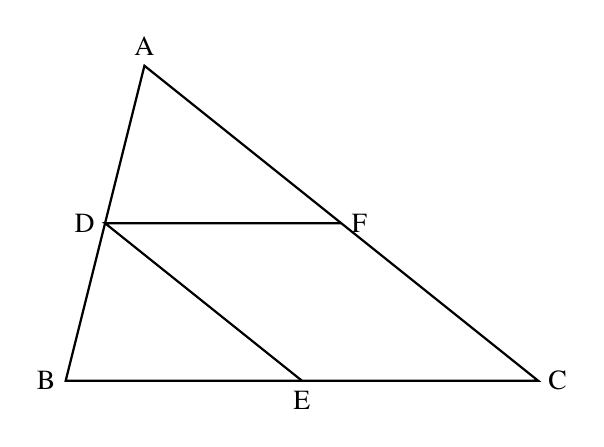
\begin{tikzpicture}[scale=1]
				\coordinate(b) at (0, 0);
				\coordinate(a) at (1, 4);
				\coordinate(c) at (6, 0);
				
				\coordinate(d) at ($(a)!0.5!(b)$);
				\coordinate(e) at ($(c)!0.5!(b)$);
				\coordinate(f) at ($(a)!0.5!(c)$);

				\draw[thick] (a)node[above]{A}--(b)node[left]{B}--(c)node[right]{C}--cycle;
				\draw[thick] (f)node[right]{F}--(d)node[left]{D}--(e)node[below]{E};

			\end{tikzpicture}
			\caption{:$\mathrm{AD}=\mathrm{DB}, \mathrm{DF}//\mathrm{BC}, \mathrm{DF}=\mathrm{BE}$}
			\label{tizk_01_ex1}
		\end{figure}

		\qpart 図\ref{tizk_01_ex2}で $\mathrm{DF}//\mathrm{BC}, \mathrm{DE}//\mathrm{AC}$である.
		このときに次の問に答えよ.

		\begin{qlist}
			\qitem $\triangle\mathrm{FEC}\equiv\triangle\mathrm{EFD}$を示せ.
			\qitem $\triangle\mathrm{DEF}$の面積が1であるとき,
			$\triangle\mathrm{ABC}$の面積がどうなるのか答えよ.
		\end{qlist}

		\begin{figure}[htbp]
			\centering
			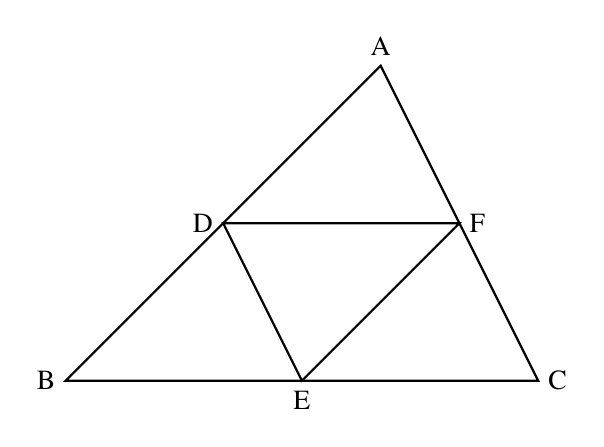
\begin{tikzpicture}[scale=1]
				\coordinate(b) at (0, 0);
				\coordinate(a) at (4, 4);
				\coordinate(c) at (6, 0);
				
				\coordinate(d) at ($(a)!0.5!(b)$);
				\coordinate(e) at ($(c)!0.5!(b)$);
				\coordinate(f) at ($(a)!0.5!(c)$);

				\draw[thick] (a)node[above]{A}--(b)node[left]{B}--(c)node[right]{C}--cycle;
				\draw[thick] (f)node[right]{F}--(d)node[left]{D}--(e)node[below]{E}--(f)--cycle;

			\end{tikzpicture}
			\caption{:$\mathrm{DF}//\mathrm{BC}, \mathrm{DE}//\mathrm{AC}$}
			\label{tizk_01_ex2}
		\end{figure}

	\end{qparts}

\end{document}
